\begin{figure}[!ht]
    \centering
    \resizebox{\columnwidth}{!}{
    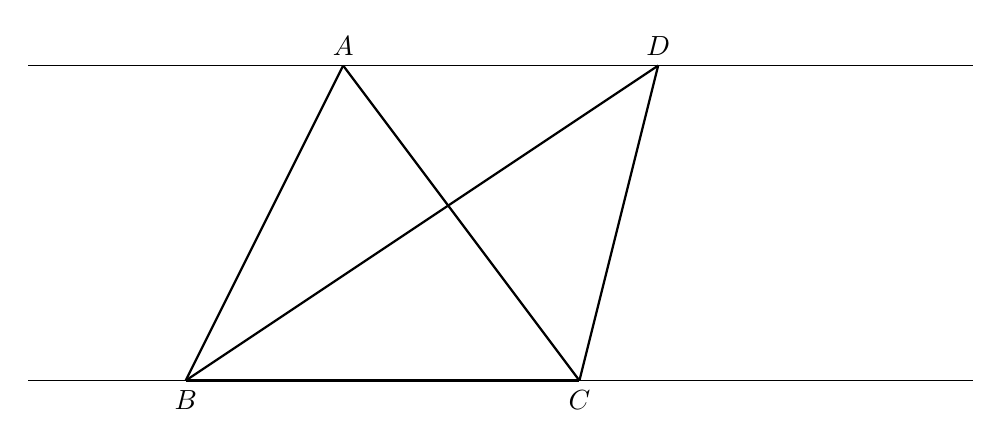
\begin{tikzpicture}
        \draw (-2,0) -- (10,0); 
        \draw (-2,4) -- (10,4);
        \filldraw[black] (0,0) node[anchor=north] {$B$};
        \filldraw[black] (2,4) node[anchor=south] {$A$};
        \filldraw[black] (5,0) node[anchor=north] {$C$};
        \filldraw[black] (6,4) node[anchor=south] {$D$};
        \draw[black,thick] (0,0) -- (2,4);
        \draw[black,thick] (0,0) -- (5,0);
        \draw[black,thick] (5,0) -- (2,4);
        \draw[black,thick] (0,0) -- (6,4);
        \draw[black,thick] (5,0) -- (6,4);
    \end{tikzpicture}}
    \caption{$\triangle{ABC}$ and $\triangle{BCD}$ having common base $BC$}
    \label{eq:solutions/1/14/fig:solutions/1/14/triangle}
\end{figure}
Given that, 
\begin{equation}
    \label{eq:solutions/1/14/eq1}\text{Area of }\triangle{ABC} = \text{Area of }\triangle{BCD}
\end{equation}
We know that, area of triangle can be obtained by cross product.
{\small
\begin{align}
    \text{Area of }\triangle{ABC} 
    \label{eq:solutions/1/14/eq2}&= \frac{1}{2} \norm{(\vec{B}-\vec{A}) \times (\vec{B}-\vec{C})}\\
    \label{eq:solutions/1/14/eq3}&= \frac{1}{2} \norm{\big((\vec{B}-\vec{D})+(\vec{D}-\vec{A})\big) \times (\vec{B}-\vec{C})}\\
    \label{eq:solutions/1/14/eq4}&= \text{Area of }\triangle{BCD} + \frac{1}{2} \norm{(\vec{D}-\vec{A}) \times (\vec{B}-\vec{C})}
\end{align}
}
From \eqref{eq:solutions/1/14/eq1} and \eqref{eq:solutions/1/14/eq4} we get,
\begin{equation}
    \label{eq:solutions/1/14/eq5}\norm{(\vec{D}-\vec{A}) \times (\vec{B}-\vec{C})} = 0
\end{equation}
We know that, two nonzero vectors are \textbf{parallel} if and only if their cross product is zero.
\begin{equation}
    \label{eq:solutions/1/14/eq6}\implies (\vec{A}-\vec{D}) = k(\vec{B}-\vec{C})
\end{equation}
Hence proved triangles on the same base and having equal areas lie between the same parallels.
